\chapter{Parallelisierungsstrategien}

Aufgrund seiner einfachen Implementierbarkeit ist der \gls{fdk} einer der beliebtesten Rückprojektionsalgorithmen für
die Kegelstrahl-Computertomographie. Ein Vorteil des \gls{fdk} liegt außerdem darin, dass die gefilterte Rückprojektion
für jedes \gls{voxel} individuell berechnet werden kann, das heißt ohne Abhängigkeiten zu anderen \gls{voxel}n. Dieser
Umstand ermöglicht für die maschinelle Berechnung den maximalen Grad an Parallelität, der im englischen Sprachraum auch
als \textit{embarassingly parallel} bezeichnet wird, und macht den \gls{fdk} zu einem idealen Ziel für diverse
Parallelisierungsansätze. Einige neuere Ansätze sollen im Folgenden vorgestellt werden. Aus einem Variantenvergleich
der auf dem Einsatz von \gls{gpu}s basierenden Ideen wird dann ein eigener Implementierungsvorschlag entwickelt.

\section{Forschungsstand}\label{sec:forschungsstand}

Xu et al.\ untersuchten bereits 2004, inwieweit sich der \gls{fdk} durch den Einsatz handelsüblicher Grafikkarten
(\textit{commodity graphics hardware}) beschleunigen lässt. Dabei wurden die Schritte \textit{Wichtung} und
\textit{Filterung} aufgrund ihrer geringen Komplexität ($\mathcal{O}(n^2)$) auf der \gls{cpu} ausgeführt, während man
die komplexere \textit{Rückprojektion} ($\mathcal{O}(n^4)$) auf der \gls{gpu} berechnete. Die Rückprojektion fand
schichtweise statt, jeweils für eine \gls{voxel}ebene entlang der vertikalen Volumenachse. In ihrem Fazit stellten die
Autoren die Vermutung auf, dass der Abstand zwischen den Leistungen von \gls{cpu}s und \gls{gpu}s in der Zukunft
zugunsten der \gls{gpu}s immer größer werden würde: \textit{Since GPU performance has so far doubled every 6 months 
(i.e., triple of Moore's law), we expect that the gap between CPU and GPU approaches will widen even further in the near
future.} (vgl.~\cite{xumuell})

Li et al.\ beschäftigten sich 2005 damit, wie man den \gls{fdk} mit einem \gls{fpga} implementieren könnte. Dazu teilten
sie das Ausgabevolumen, also die Zieldaten der Rückprojektion, in mehrere Würfel (\textit{bricks}) auf, um zu einer
optimalen Cachenutzung zu kommen. Der verwendete deterministische Aufteilungsalgorithmus hatte zur Folge, dass bei der
Berechnung auf dem \gls{fpga} kein Cache-Verfehlen (\textit{cache miss}) mehr auftrat. (vgl.~\cite{lipapa})

Knaup et al.\ gingen 2007 der Frage nach, ob die Parallelisierung des \gls{fdk} durch die Eigenschaften der
Cell-Architektur profitieren könne. (vgl.~\cite{knaupsteck})

Scherl et al.\ unternahmen 2008 den Versuch, den \gls{fdk} mittels \gls{cuda} zu beschleunigen. Im Gegensatz zu der
Gruppe um Xu et al.\ führten sie alle Schritte auf der \gls{gpu} aus und führten die Rückprojektion projektionsweise
durch, das heißt, dass jede Projektion einzeln in das Gesamtvolumen zurückprojiziert wurde. Diese Art der
Datenverarbeitung ermöglichte es, die Schritte \textit{Wichtung} und \textit{Filterung} parallel zur Rückprojektion
auszuführen (vgl.~\cite{scherlkeck}). Zur Ausnutzung dieser Eigenschaft und zur besseren Kapselung bzw.\ Modularisierung
der Teilschritte entwickelten die Autoren daher eine Pipeline-Struktur zur parallelen Abarbeitung des Algorithmus,
basierend auf dem von Mattson et al.\ vorgestellten Entwurfsmuster (vgl.~\cite{mattsan}).

Hofmann et al.\ untersuchten 2013 eventuelle Vorteile durch den Einsatz der neuen Koprozessoren vom Typ Intel Xeon Phi
{\glq}Knights Corner{\grq}. Der Fokus ihrer Arbeit lag dabei auf dem Ausnutzen architektonischer Details des Xeon Phi,
wie etwa effizienter Vektorregister-Operationen. (vgl.~\cite{hoftrei})

Zhao et al.\ verfolgten die Absicht, eine Beschleunigung durch Ausnutzung geometrischer Zusammenhänge zu
erreichen. Sie setzten dabei auf die Tatsache, dass ein einmal bestimmtes, also auf den Detektor projiziertes,
\gls{voxel} durch Rotation in 90-Grad-Schritten die rotierten \gls{voxel} ebenfalls genau bestimmt. Ist also für ein
\gls{voxel} im Projektionswinkel 0 Grad die zugehörige Detektorkoordinate gefunden, so kann diese Detektorkoordinate für
die Projektionswinkel 90 Grad, 180 Grad und 270 Grad und die entsprechenden \gls{voxel} wiederverwendet werden.
(vgl.~\cite{zhao})

\section{Variantenvergleich}

Von den vorgestellten Parallelisierungsansätzen sind für diese Arbeit vor allem die \gls{gpu}-Implementierungen von
besonderem Interesse. Diese weisen allerdings einige Schwächen auf, die im Folgenden vorgestellt werden. Erläutert
werden außerdem das Problem des begrenzten \gls{gpu}-Speichers, der allen Ansätzen gemein ist, sowie dessen Abschwächung
durch den Einsatz mehrerer \gls{gpu}s. Eine Möglichkeit der Parallelisierung des \gls{fdk}, die auf den vorgestellten
Ansätzen und Problemen und daraus gezogenen Schlüssen aufbaut, schließt das Kapitel ab.

\subsection{Bestehende Parallelisierungsstrategien und ihre Grenzen}\label{ssec:par_strat}

Von den in Abschnitt~\ref{sec:forschungsstand} genannten Ansätzen in der Literatur sind aufgrund ihrer Umsetzung für
\gls{gpu}s die Strategien von Xu et al. (vgl.~\cite{xumuell}), Scherl et al. (vgl.~\cite{scherlkeck}) und Zhao et al.
(vgl.~\cite{zhao}) von besonderem Interesse für diese Arbeit.

Da Xu et al. 2004 mit ihrer Arbeit Neuland betraten, standen ihnen viele Methoden und Technologien, die seitdem 
entwickelt wurden, noch nicht zur Verfügung. Die 2004 erschienenen \gls{gpu}s hatten im Vergleich zu heutigen
Grafikkarten sehr viel weniger Speicher; das damals beste verfügbare Produkt von NVIDIA, die GeForce 6800 Ultra, konnte
lediglich mit 512 MiB Speicher aufwarten und war nur über die \gls{opengl} oder \gls{directx} indirekt programmierbar.
Den begrenzten Speicher versuchte die Gruppe durch eine Aufteilung des Volumens und eine schichtweise Rekonstruktion
desselben unter Einbeziehung aller Projektionen möglichst effizient zu nutzen (vgl.~\cite{xumuell}). Aufgrund des
technischen Fortschritts gibt es heute andere Möglichkeiten zur Lösung dieses Problems; so bietet etwa die NVIDIA
GeForce GTX 1080 mit 8 GiB Speicher und der Möglichkeit der direkten Programmierung mittels \gls{cuda} oder
der \gls{opencl} ganz andere Nutzungs- und Berechnungsmöglichkeiten als ihre frühen Vorgänger. Insbesondere ist es
möglich, das ganze Volumen oder größere Teile davon während der Berechnung im Speicher zu halten und dadurch häufige
Kopien zwischen \gls{cpu}-Speicher und \gls{gpu}-Speicher zu vermeiden.

Die Forschungsgruppe um Scherl baute auf der Idee, das Volumen im Speicher zu halten, auf und ging im Gegensatz zu Xu et
al.\ den Weg, jede Projektion einzeln in dieses Volumen zu projizieren (vgl.~\cite{scherlkeck}). Zur Trennung bzw.\
Kapselung der einzelnen Schritte entwickelten sie in einem vorherigen Schritt (vgl.~\cite{scherlhopp}) eine
Pipeline-Struktur (nach Mattson et al., vgl.~\cite{mattsan}). Jeder Schritt des \gls{fdk} wird dabei in einer eigenen
Stufe (\textit{stage}) ausgeführt, die in einem separaten Thread ausgeführt wird. Zur Kommunikation der Ergebnisse der
einzelnen Stufen werden thread-sichere Puffer verwendet, auf die die Eingabe- bzw.\ Ausgaberoutinen der Stufen
zugreifen. Die eigentliche Rekonstruktion erfolgt entlang der $z$-Achse und der $y$-Achse: Jede $z$-Schicht im Volumen
wird entlang der $x$-Achse nocheinmal in Spalten aufgeteilt. Ein zweidimensionaler \gls{kernel} iteriert dann über alle
\gls{voxel} in $y$-Richtung (vgl. Abbildung~\ref{fig:scherl}). Der Nachteil des von Scherl et al.\ gewählten Ansatzes
liegt in der Pipeline-Struktur, die durch die wesentlich längere Laufzeit der Rückprojektion nicht optimal ist. So
schreiben Mattson et al.: {\glqq}If the stages in the pipeline vary widely in computational effort, the slowest stage
creates a bottleneck for the aggregate throughput{\grqq} (\cite{mattsan}, S. 106).

Die Grenzen bei dem vorgeschlagenen Verfahren der Gruppe um Zhao et al.\ sind vor allem praktischer Natur. Das von ihnen
vorgestellte Modell sieht vor, Symmetrien auszunutzen und dadurch Rechenzeit einzusparen (vgl.\
Abbildung~\ref{fig:zhao}). Sie machen sich dabei den Umstand zunutze, dass die auf den Detektor projizierte Koordinate
eines \gls{voxel}s der um 90 Grad rotierten Projektionskoordinate des um den gleichen Betrag rotierten Voxels
entspricht. Auf diese Weise lassen sich durch eine Berechnung die Detektorkoordinaten von vier \gls{voxel}n finden, was
eine Verkürzung der Rechenzeit verspricht (vgl.~\cite{zhao}). In der Praxis scheitert dieses Verfahren an dem
mechanischen Aufbau üblicher CT-Scanner. Da entweder Quelle und Detektor oder aber das Untersuchungsobjekt rotiert
werden müssen, kommt es durch Fehler in der Mechanik häufig dazu, dass Aufnahmen doppelt gemacht oder übersprungen
werden, sodass die für die Nutzung der Symmetrien nötigen Projektionen fehlen.

\begin{figure}[!htb]
    \centering
    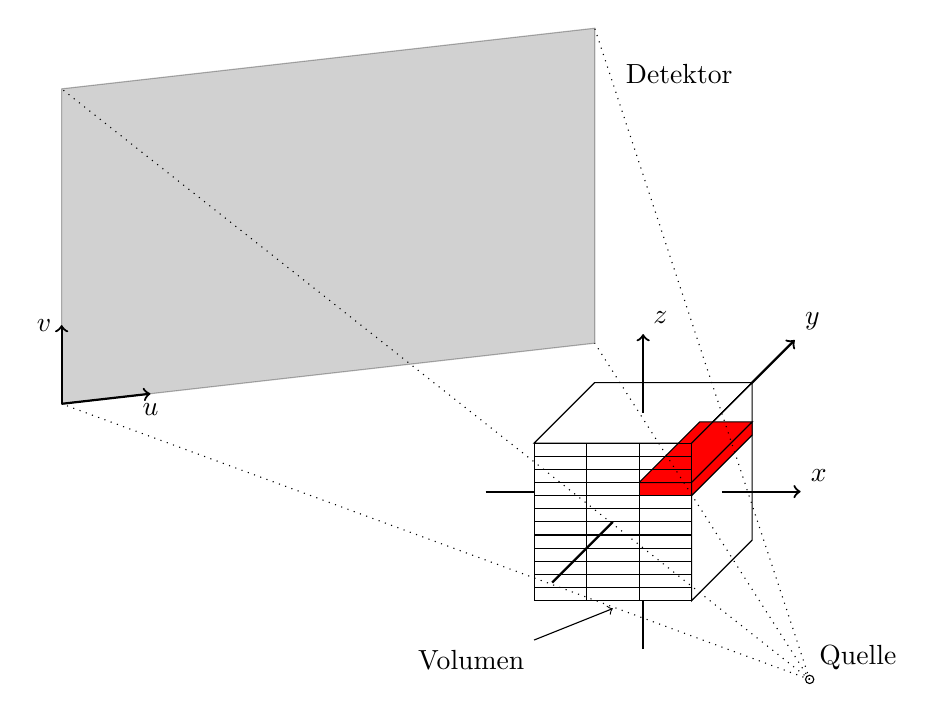
\begin{tikzpicture}[axis/.style={thick,->}]
        \draw[fill=black!60!white,opacity=0.3] (0, 0, 0) -- (0, 4, 0) -- (6, 4, -2) -- (6, 0, -2) -- (0, 0, 0);
        \draw[axis] (0, 0, 0) -- (0, 1, 0) node[left] {$v$};
        \draw[axis] (0, 0, 0) -- (1, 0, -0.33333333) node[below] {$u$};

        % Achsenanfang
        \draw[thick] (5, -1.5, -1) -- (6, -1.5, -1); % x
        \draw[axis] (7, -1.5, -2) -- (7, -1.5, -6) node[above right] {$y$}; % y
        \draw[thick] (7, -3.5, -1) -- (7, -2.5, -1); % z

        % Volumen
        \draw[fill=white] (6, -0.5, -2) -- (8, -0.5, -2) -- (8, -0.5, 0) -- (6, -0.5, 0) -- (6, -0.5, -2);
        \draw[fill=white] (6, -0.5, 0) -- (8, -0.5, 0) -- (8, -2.5, 0) -- (6, -2.5, 0) -- (6, -0.5, 0);
        \draw[fill=white] (8, -0.5, -2) -- (8, -2.5, -2) -- (8, -2.5, 0) -- (8, -0.5, 0) -- (8, -0.5, -2);

        \draw[->] (6, -3, 0) -- (7, -2.6, 0) node[pos=0,below left] {Volumen};

        % Achsenende
        \draw[axis] (8, -1.5, -1) -- (9, -1.5, -1) node[above right] {$x$}; % x
        \draw[thick] (7, -1.5, 2) -- (7, -1.5, 0); % y
        \draw[axis] (7, -0.5, -1) -- (7, 0.5, -1) node[above right] {$z$}; % z

        % Teilvolumen
        \draw[fill=red] (7.333333, -1, 0) -- (8, -1, 0) -- (8, -1.166666, 0) -- (7.333333, -1.166666, 0)
                        -- (7.333333, -1, 0);
        \draw[fill=red] (7.333333, -1, 0) -- (7.333333, -1, -2) -- (8, -1, -2) -- (8, -1, 0) -- (7.333333, -1, 0);
        \draw[fill=red] (8, -1, 0) -- (8, -1, -2) -- (8, -1.166666, -2) -- (8, -1.166666, 0) -- (8, -1, 0);

        \draw (6.666666, -0.5, 0) -- (6.666666, -2.5, 0); % v1
        \draw (7.333333, -0.5, 0) -- (7.333333, -2.5, 0); % v2
        \draw (6, -0.666666, 0) -- (8, -0.666666, 0); % h1
        \draw (6, -0.833333, 0) -- (8, -0.833333, 0); % h2
        \draw (6, -1, 0) -- (8, -1, 0); % h3
        \draw (6, -1.166666, 0) -- (8, -1.166666, 0); % h4
        \draw (6, -1.333333, 0) -- (8, -1.333333, 0); % h5
        \draw (6, -1.5, 0) -- (8, -1.5, 0); % h6
        \draw (6, -1.666666, 0) -- (8, -1.666666, 0); % h7
        \draw (6, -1.833333, 0) -- (8, -1.833333, 0); % h8
        \draw (6, -2, 0) -- (8, -2, 0); % h9
        \draw (6, -2.166666, 0) -- (8, -2.166666, 0); % h10
        \draw (6, -2.333333, 0) -- (8, -2.333333, 0); % h11

        % fehlende Linien nachzeichnen
        \draw (8, -0.5, 0) -- (8, -0.5, -2);
        \draw (8, -0.5, 0) -- (8, -2.5, 0);
        \draw (6, -0.5, 0) -- (8, -0.5, 0);

        % Quelle und Kegelstrahl
        \coordinate (s) at (9.5, -3.5, 0);
        \draw (s) circle (1.5pt) node[above right] {Quelle};
        \draw[dotted] (s) -- (0, 0, 0);
        \draw[dotted] (s) -- (0, 4, 0);
        \draw[dotted] (s) -- (6, 4, -2) node[pos=0.9,above right] {Detektor};
        \draw[dotted] (s) -- (6, 0, -2);
    \end{tikzpicture}
    \captionof{figure}{Aufteilung des Volumens nach Scherl et al. (Vorlage:~\cite{scherlkeck})}
    \label{fig:scherl}
\end{figure}

\begin{figure}[!htb]
    \centering
    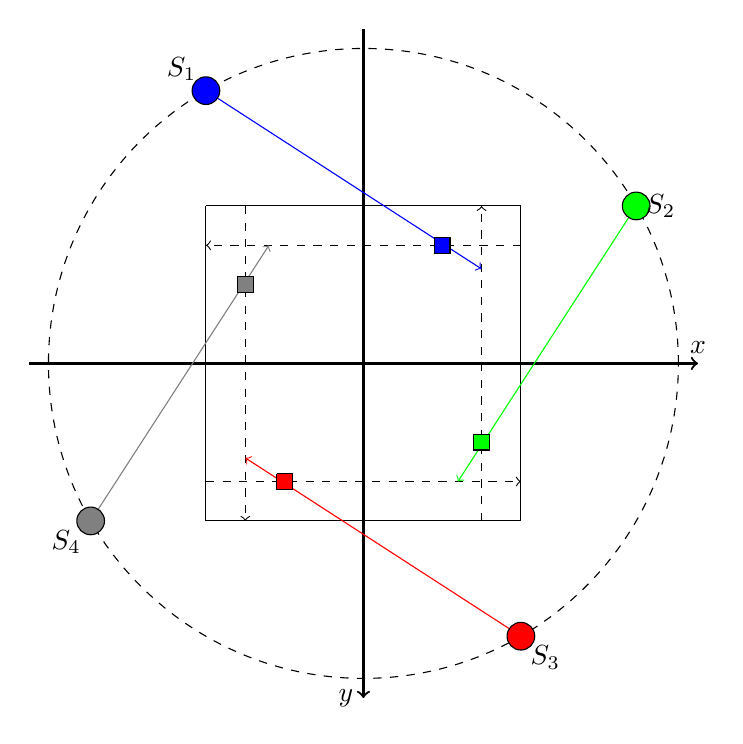
\begin{tikzpicture}[axis/.style={thick,->}]
        \draw[axis] (0, 4.25, 0) -- (0, -4.25, 0) node [left] {$y$};
        \draw[axis] (-4.25, 0, 0) -- (4.25, 0, 0) node [above] {$x$};

        % Volumen
        \draw (-2, 2, 0) -- (2, 2, 0) -- (2, -2, 0) -- (-2, -2, 0) -- (-2, 2, 0);

        % Pfeile im Volumen
        \draw[dashed,->] (-1.5, 2, 0) -- (-1.5, -2, 0);
        \draw[dashed,->] (2, 1.5, 0) -- (-2, 1.5, 0);
        \draw[dashed,->] (1.5, -2, 0) -- (1.5, 2, 0);
        \draw[dashed,->] (-2, -1.5, 0) -- (2, -1.5, 0);

        % Kreis
        \draw[dashed] (0, 0, 0) circle [radius=4];

        % Quellpfeile
        \draw[color=blue,->] (-2, 3.46410) -- (1.5, 1.2);
        \draw[color=green,->] (3.46410, 2) -- (1.2, -1.5);
        \draw[color=red,->] (2, -3.46410) -- (-1.5, -1.2);
        \draw[color=gray,->] (-3.46410, -2) -- (-1.2, 1.5);

        % Quellpositionen
        \draw[fill=blue] (-2, 3.46410) circle (5pt) node [above left] {$S_1$};
        \draw[fill=green] (3.46410, 2) circle (5pt) node [right] {$S_2$};
        \draw[fill=red] (2, -3.46410) circle (5pt) node [below right] {$S_3$};
        \draw[fill=gray] (-3.46410, -2) circle (5pt) node [below left] {$S_4$};

        % Voxel
        \draw[fill=blue] (0.9, 1.6) -- (1.1, 1.6) -- (1.1, 1.4) -- (0.9, 1.4) -- (0.9, 1.6);
        \draw[fill=green] (1.4, -0.9) -- (1.6, -0.9) -- (1.6, -1.1) -- (1.4, -1.1) -- (1.4, -0.9);
        \draw[fill=red] (-1.1, -1.4) -- (-0.9, -1.4) -- (-0.9, -1.6) -- (-1.1, -1.6) -- (-1.1, -1.4);
        \draw[fill=gray] (-1.6, 1.1) -- (-1.4, 1.1) -- (-1.4, 0.9) -- (-1.6, 0.9) -- (-1.6, 1.1);
    \end{tikzpicture}
    \captionof{figure}{Symmetrien bei der Rückprojektion nach Zhao et al. (Vorlage:~\cite{zhao})}
    \label{fig:zhao}
\end{figure}

\subsection{Begrenzter GPU-Speicher}

Den oben vorgestellten Ansätzen ist gemein, dass sie alle mit dem limitierten Speicher einer \gls{gpu} arbeiten mussten.
Während der technische Fortschritt die Speichergrenze seitdem weiter nach oben verschoben hat, hat sich das
zugrundeliegende Problem dennoch nicht wesentlich verändert. Mit modernen \gls{gpu}s wie der NVIDIA GeForce GTX 1080 ist
es inzwischen zwar möglich, komplette Volumen oder wenigstens große Teile davon während der Rückprojektion im
\gls{gpu}-Speicher zu halten und so die Zahl der Kopien zwischen \gls{host} und \gls{device} zu reduzieren; der parallel
stattfindende Fortschritt bei der Computertomographie, insbesondere im Hinblick auf die Detektorauflösung und die
dadurch produzierte Datenmenge, erhöht allerdings auch weiterhin den für die Berechnung erforderlichen Speicher. Im
Gegensatz zu den klassischen \gls{cpu}s, deren Speicher sich theoretisch nahezu unbegrenzt erhöhen lässt, ist für die
Parallelisierung mit \gls{gpu}s eine Strategie zur Verwaltung des zur Verfügung stehenden Speichers also weiterhin
unabdingbar.

\subsection{Heterogene GPU-Systeme und effiziente Arbeitsteilung}

Ein naheliegender Weg zur Umgehung des begrenzten \gls{gpu}-Speichers ist der parallele Einsatz mehrerer \gls{gpu}s.
Dieser Ansatz wirft jedoch einige neue Probleme auf.

Am vordringlichsten ist die Frage zu beantworten, in welcher Form die Berechnung auf die verfügbaren \gls{gpu}s verteilt
werden soll. Während dies für den Fall, dass mehrere gleichartige \gls{gpu}s verwendet werden sollen, relativ einfach
ist, wird die Lastverteilung beim Einsatz unterschiedlich leistungsstarker Grafikkarten deutlich schwieriger. Es ist zu
vermeiden, dass die schnelleren \gls{gpu}s auf die langsameren warten müssen, da so Rechenzeit verschenkt wird.

In beiden Fällen kommt hinzu, dass die vorhandenen Grafikkarten möglichst parallel mit Daten befüllt und zur Berechnung
gebracht werden sollen, die vorgesehenen Schritte der Rückprojektion also weitestgehend gleichzeitig ausgeführt werden.

\subsection{Implementierungsidee}\label{ssec:implementierungsidee}

Aus den oben genannten Faktoren beim Einsatz von \gls{gpu}s ergeben sich die folgenden Anforderungen an eine effiziente
Parallelisierungsstrategie des \gls{fdk}:

\begin{enumerate}
    \item der auf \gls{gpu}s beschränkte Speicher muss möglichst effizient genutzt werden, häufige Kopien sollten also
          vermieden werden.
    \item Die Optimierung der Rückprojektionen sollte die höchste Priorität genießen, woraus folgt, dass
    \item die Rückprojektion die zur Verfügung stehenden \gls{gpu}s möglichst stark auslasten sollte.
    \item Die Wartezeit zwischen zwei Rückprojektionen sollte möglichst minimal sein, um die \gls{gpu} nicht
          unnötigerweise geringer auszulasten.
    \item Die Parallelisierung sollte sich über mehrere \gls{gpu}s skalieren lassen.
\end{enumerate}

Mit der Umsetzung der Punkte 2.\ und 3.\ beschäftigt sich detailliert das nächste Kapitel, ein Lösungsvorschlag für
die restlichen Punkte findet sich in der im Folgenden skizzierten Programmstruktur.

Ein üblicher Projektionsdatensatz umfasst 1440 Projektionen, die jeweils eine Auflösung von 1024 x 1024 \gls{pixel}n
haben; jeder Pixel ist dabei im 4-Byte-Fließkommazahlen-Format gespeichert. Für den kompletten Datensatz ergibt sich
dadurch eine Datenmenge von 5,625 GiB. Das daraus resultierende Volumen besitzt (abhängig von den konkreten
Geometrieparametern der CT-Anlage) etwa 1070 $\times$ 1070 $\times$ 1033 \gls{voxel} (vgl.
Abschnitt~\ref{ssec:geometrie}), die das gleiche Datenformat wie die Pixel aufweisen. Die Datengröße des Volumens
beträgt 4,4 GiB und die kumulierte Datenmenge damit 10,25 GiB. Ausgehend von der Annahme, dass eine \gls{gpu} des Typs
GeForce GTX 1080 zur Verfügung steht, ist der vorhandene Speicher schon für die zu verarbeitenden Daten nicht
ausreichend, da diese \gls{gpu} lediglich 8 GiB Speicher besitzt. Sowohl die Projektionen als auch das komplette Volumen
im Speicher zu halten ist demnach kein praktikabler Ansatz. In Abschnitt~\ref{ssec:par_strat} wurden mehrere Ansätze der
Literatur vorgestellt, die dieses Problem zu umgehen versuchen.

Der erste Ansatz von Xu et al.\ sieht eine Aufteilung des Volumens in mehrere Segmente vor. Jedes Teilvolumen wird dann
durch die Iteration über den kompletten Projektionsdatensatz berechnet (vgl.~\cite{xumuell}). Allerdings muss bei diesem
Ansatz zusätzlich zur Aufteilung des Volumens ein Weg gefunden werden, alle Projektionen effizient auf der \gls{gpu}
abzubilden, da -- wie oben gezeigt -- der Projektionsdatensatz tendenziell größer ist als das komplette Volumen. Dies
erzeugt zusätzliche Komplexität und damit unerwünschten \textit{Overhead}.

Scherl et al.\ schlagen den umgekehrten Weg vor, sodass das ganze Volumen bzw.\ ein möglichst großer Teil davon im
Speicher gehalten wird. Die Projektionen werden dann einzeln geladen und in das Volumen zurückprojiziert
(vgl.~\cite{scherlkeck}). Gegenüber der von Xu et al.\ gewählten Variante bietet dies den Vorteil, dass nicht mehr alle
Projektionen im Speicher gehalten werden bzw.\ im richtigen Iterationsschritt vorhanden sein müssen; stattdessen werden
die Projektionen sequentiell geladen und verarbeitet. Im idealen Fall (das ganze Volumen passt in den Speicher) entfällt
zudem die Notwendigkeit für Teilvolumen, sodass es genau einen Kopiervorgang bezüglich des Volumens am Ende der
Berechnung gibt.

Für den Fall, dass das Volumen nicht in Gänze in den \gls{gpu}-Speicher passt, schlagen Zhao et al.\ eine Aufteilung
entlang der $z$-Achse vor (vgl.~\cite{zhao}). Das Volumen wird dabei in $N$ gleich große Teilvolumen zerlegt, die
einzeln in den \gls{gpu}-Speicher passen. Jede Projektion wird dann ebenfalls in $N$ Teilprojektionen unterteilt, sodass
jede Teilprojektion geometrisch einem Teilvolumen entspricht. Dieser Ansatz hat jedoch den Nachteil, dass die für das
aktuell zu rekonstruierende Teilvolumen nicht benötigten Teilprojektionen verwaltet bzw.\ zwischengespeichert werden
müssen, was ebenfalls zusätzliche Komplexität in den Algorithmus einführt.

Aufgrund der geschilderten Vorteile im Hinblick auf den begrenzt verfügbaren \gls{gpu}-Speicher ist es daher sinnvoll,
dem Ansatz von Scherl et al.\ zu folgen und die Rückprojektion sequentiell für jede Projektion durchzuführen, während
das ganze Volumen im Speicher gehalten wird. Sollte der vorhandene Speicher nicht ausreichen, muss das Volumen
in mehrere Teilvolumen zerlegt werden, die dann einzeln rekonstruiert und zum Schluss wieder zusammengesetzt werden.
Abweichend von Zhao et al.\ ist eine entsprechende Unterteilung der Projektionen aus zweierlei Gründen nicht notwendig.
Einerseits besitzt eine einzelne Projektion des obigen Beispiels eine im Vergleich zum Volumen vernachlässigbare
Datengröße von 4 MiB, sodass der durch eine Aufteilung eingesparte Speicher keinen nennenswerten Mehrwert bietet,
andererseits ist der Zeitaufwand der Wichtungs- und Filteroperationen verglichen mit der Rückprojektion derart gering,
dass die Durchführung dieser Operationen auf weniger Pixeln in Bezug auf die Gesamtlaufzeit keine bemerkenswerte
Zeitersparnis verspricht. Es ist hierbei zu beachten, dass dadurch alle Projektionen für jedes Teilvolumen neu geladen
werden müssen, sobald die Berechnung des vorherigen Teilvolumens abgeschlossen ist. Bei einer Datenübertragung über das
Netzwerk oder einer langsamen Festplatte kann sich dieser Faktor schnell zu einem Flaschenhals entwickeln, sofern der
(gegebenenfalls gewichtete und gefilterte) Projektionsdatensatz nicht auf andere Art und Weise zwischengespeichert
werden kann.

Eine weitere Herausforderung ist die Minimierung der Wartezeit zwischen zwei aufeinanderfolgenden Rückprojektionen.
Theoretisch wäre es hier denkbar, zwei oder mehr Rückprojektionen verschiedener Projektionen gleichzeitig durchzuführen.
Praktisch ergäbe sich daraus die Notwendigkeit der Synchronisierung zwischen den verschiedenen
Rückprojektionsoperationen, um Datenkorruption durch \textit{\glspl{race-condition}} zu vermeiden. Es ist daher der
einfachere Weg, die Rückprojektionen in sequentieller Reihenfolge durchzuführen. Um die Wartezeiten zwischen zwei
Rückprojektionen zu minimieren, sollten möglichst keine weiteren Operationen in der Zwischenzeit ausgeführt werden.
Idealerweise werden dann -- neben der Rückprojektion selbst -- nur noch das Entnehmen der aktuellen Projektion vom
Eingabepuffer sowie das Übergeben dieser Projektion an den Rückprojektions-\gls{kernel} ausgeführt. Demzufolge muss die
beschriebene Ausführungskette in einem eigenen Thread ausgeführt werden, um die restlichen Operationen, insbesondere die
Wichtung und die Filterung der Projektionen, durch Nebenläufigkeiten zu kaschieren.

Schwieriger ist eine effiziente Skalierung des \gls{fdk} auf heterogenen \gls{gpu}-Systemen, also Systemen mit
unterschiedlich leistungsstarken Grafikkarten. In der Literatur gibt es in jüngerer Zeit Ansätze zur besseren
(nicht FDK-spezifischen) Lastverteilung durch den Einsatz von \textit{machine-learning}-Techniken (vgl.~\cite{linhsi}),
eine Implementierung eines solchen Verfahrens geht allerdings über den Fokus dieser Arbeit hinaus und bedarf daher einer
gesonderten Untersuchung. Für den Fall, dass der implementierte Algorithmus auf einem System mit mehreren \gls{gpu}s zum
Einsatz kommt, wird daher die zu erledigende Arbeit statisch über alle verfügbaren \gls{gpu}s verteilt. Zunächst wird
das Gesamtvolumen in $N$ gleich große Teilvolumen zerlegt, wobei $N$ die Zahl der im System vorhandenen \gls{gpu}s
bezeichnet. Ist die Zahl der Schichten im Gesamtvolumen nicht glatt durch $N$ teilbar, wird der Rest an das unterste
Teilvolumen angehängt. Im Anschluss daran wird überprüft, ob diese Teilvolumen gemeinsam mit ein wenig zusätzlichem
Puffer für Projektions- und Berechnungsdaten in den kleinsten vorhandenen \gls{gpu}-Speicher passen. Ist dies nicht der
Fall, werden alle Teilvolumen so lange durch zwei geteilt, bis die so entstandenen kleineren Teilvolumen klein genug für
den Speicher sind. Für jede vorhandene Grafikkarte wird dann ein separater Thread gestartet, der die Schritte
\textit{Projektion laden} -- \textit{Wichtung} -- \textit{Filterung} -- \textit{Rückprojektion} auf dieser \gls{gpu}
ausführt (siehe Quelltext~\ref{source:high_level_fdk}). Hierbei ist zu beachten, dass aufgrund der oben geschilderten
Vorgehensweise zur Reduktion der Wartezeiten die Rückprojektion nochmals in einem weiteren Thread läuft, sodass die
Anzahl der insgesamt gestarteten Threads $2 \cdot N$ beträgt.

\begin{code}
\begin{minted}[breaklines,breakafter=\,,fontsize=\small]{c++}
// Diese Funktion läuft in einem separaten Thread pro GPU
auto fdk(task_queue& queue, // enthält ausstehende Teilvolumen
         int device) -> void
{
    cudaSetDevice(device);

    while(!queue.empty()) // solange es unbearbeitete Teilvolumen gibt
    {
        auto t = queue.pop(); // hole Teilvolumen-Informationen
        auto s = source(...); // konfiguriere Laden der Projektionen

        auto v = make_volume(...); // erzeuge Teilvolumen auf Device

        while(!source.drained()) // für jede Projektion
        {
            auto p = source.load_next(); // lade nächste Projektion
            auto d_p = copy_h2d(p); // kopiere Projektion auf Device
            weight(d_p, ...); // wichte Projektion
            filter(d_p, ...); // filtere Projektion

            /* Rückprojektion. Startet intern einen weiteren Thread,
               der die übergebenen Projektionen weiter verarbeitet */
            backproject(d_p, v, ...);
        }

        save_subvolume(v, ...); // Teilvolumen abspeichern
    }
}     
\end{minted}
\captionof{listing}{Funktionsabfolge des implementierten FDK-Algorithmus}
\label{source:high_level_fdk}
\end{code}
